%File: formatting-instruction.tex
\documentclass[letterpaper]{article}
\usepackage{aaai16}
\usepackage{times}
\usepackage{helvet}
\usepackage{courier}
\usepackage{graphicx}
\usepackage{subcaption}
\usepackage{color}
\graphicspath{ {images/} }
\setlength{\pdfpagewidth}{8.5in}
\setlength{\pdfpageheight}{11in}
%%%%%%%%%%
% PDFINFO for PDFLATEX
% Uncomment and complete the following for metadata
\pdfinfo{
/Title Writing Tool for Social Robots
/Author (Eric Rosen, Samuel Title, John Oberlin, Stefanie Tellex)}

\newcommand{\dwnote}[1]{\textcolor{blue}{\textbf{DW: #1}}}
\newcommand{\rem}[1]{\textcolor{red}{\textbf{DW: #1}}}

%%%%%%%%%%
% Section Numbers
% Uncomment if you want to use section numbers % and change the 0 to a 1 or 2
\setcounter{secnumdepth}{0} %%%%%%%%%%
% Title, Author, and Address Information \title{Title}
\title{Writing Tool for Robots}
\author{Eric Rosen \and Samuel Title \and John Oberlin \and Stefanie Tellex\\
CS Department, Brown University, Providence, RI\\}

%%%%%%%%%%
% Body of Paper Begins
\begin{document}
\maketitle

% The file aaai.sty is the style file for AAAI Press 
% proceedings, working notes, and technical reports.
%

\begin{abstract}
Writing is a valuable tool for any social agent, from leaving notes for others to read to signing for packages. To enable robots like Baxter to write, we developed a writing tool that Baxter can grip and ungrip from its end effector. This allows Baxter, a robot that has trouble writing with its built-in hardware, to write at a high proficiency with the use of a tool, as well as be able to stop using the tool in order to perform other tasks.
\end{abstract}

\section{Introduction}
Social robots are autonomous agents that can interact with human agents through typical social behaviors. Because there are so many different tasks a social robot could be asked to do, such as object delivery or writing, it is difficult to implement all the necessary hardware onto the robot to perform these tasks effectively. Humans use tools to expand their `hardware' capabilities; this idea motivates our research. Therefore, we have built a tool that lets Baxter grip a tool to write, and ungrip it to perform other tasks.

There has been research done to create robots that draw and write \cite{calinon2005humanoid}, \cite{caballero2014development}, \cite{ex66-3}, \cite{ex67-3} and \cite{ex67-3}, but these robots either have the writing hardware built into them or they simply tape the writing utensil onto the robot. The robot is unable to switch between writing and non-writing tasks.

On the other hand, \cite{hutchinson1991novel} and \cite{ex65-3} have created patents and research into creating detachable tools for robots, but these works do not focus on social tasks. They are geared towards allowing industrial robots to use different tools needed to work in a factory setting. Our research looks to mix the social aspect of the first body of work with the modularity of the second.



\begin{figure}[t]
\centering
\begin{subfigure}{.48\linewidth}
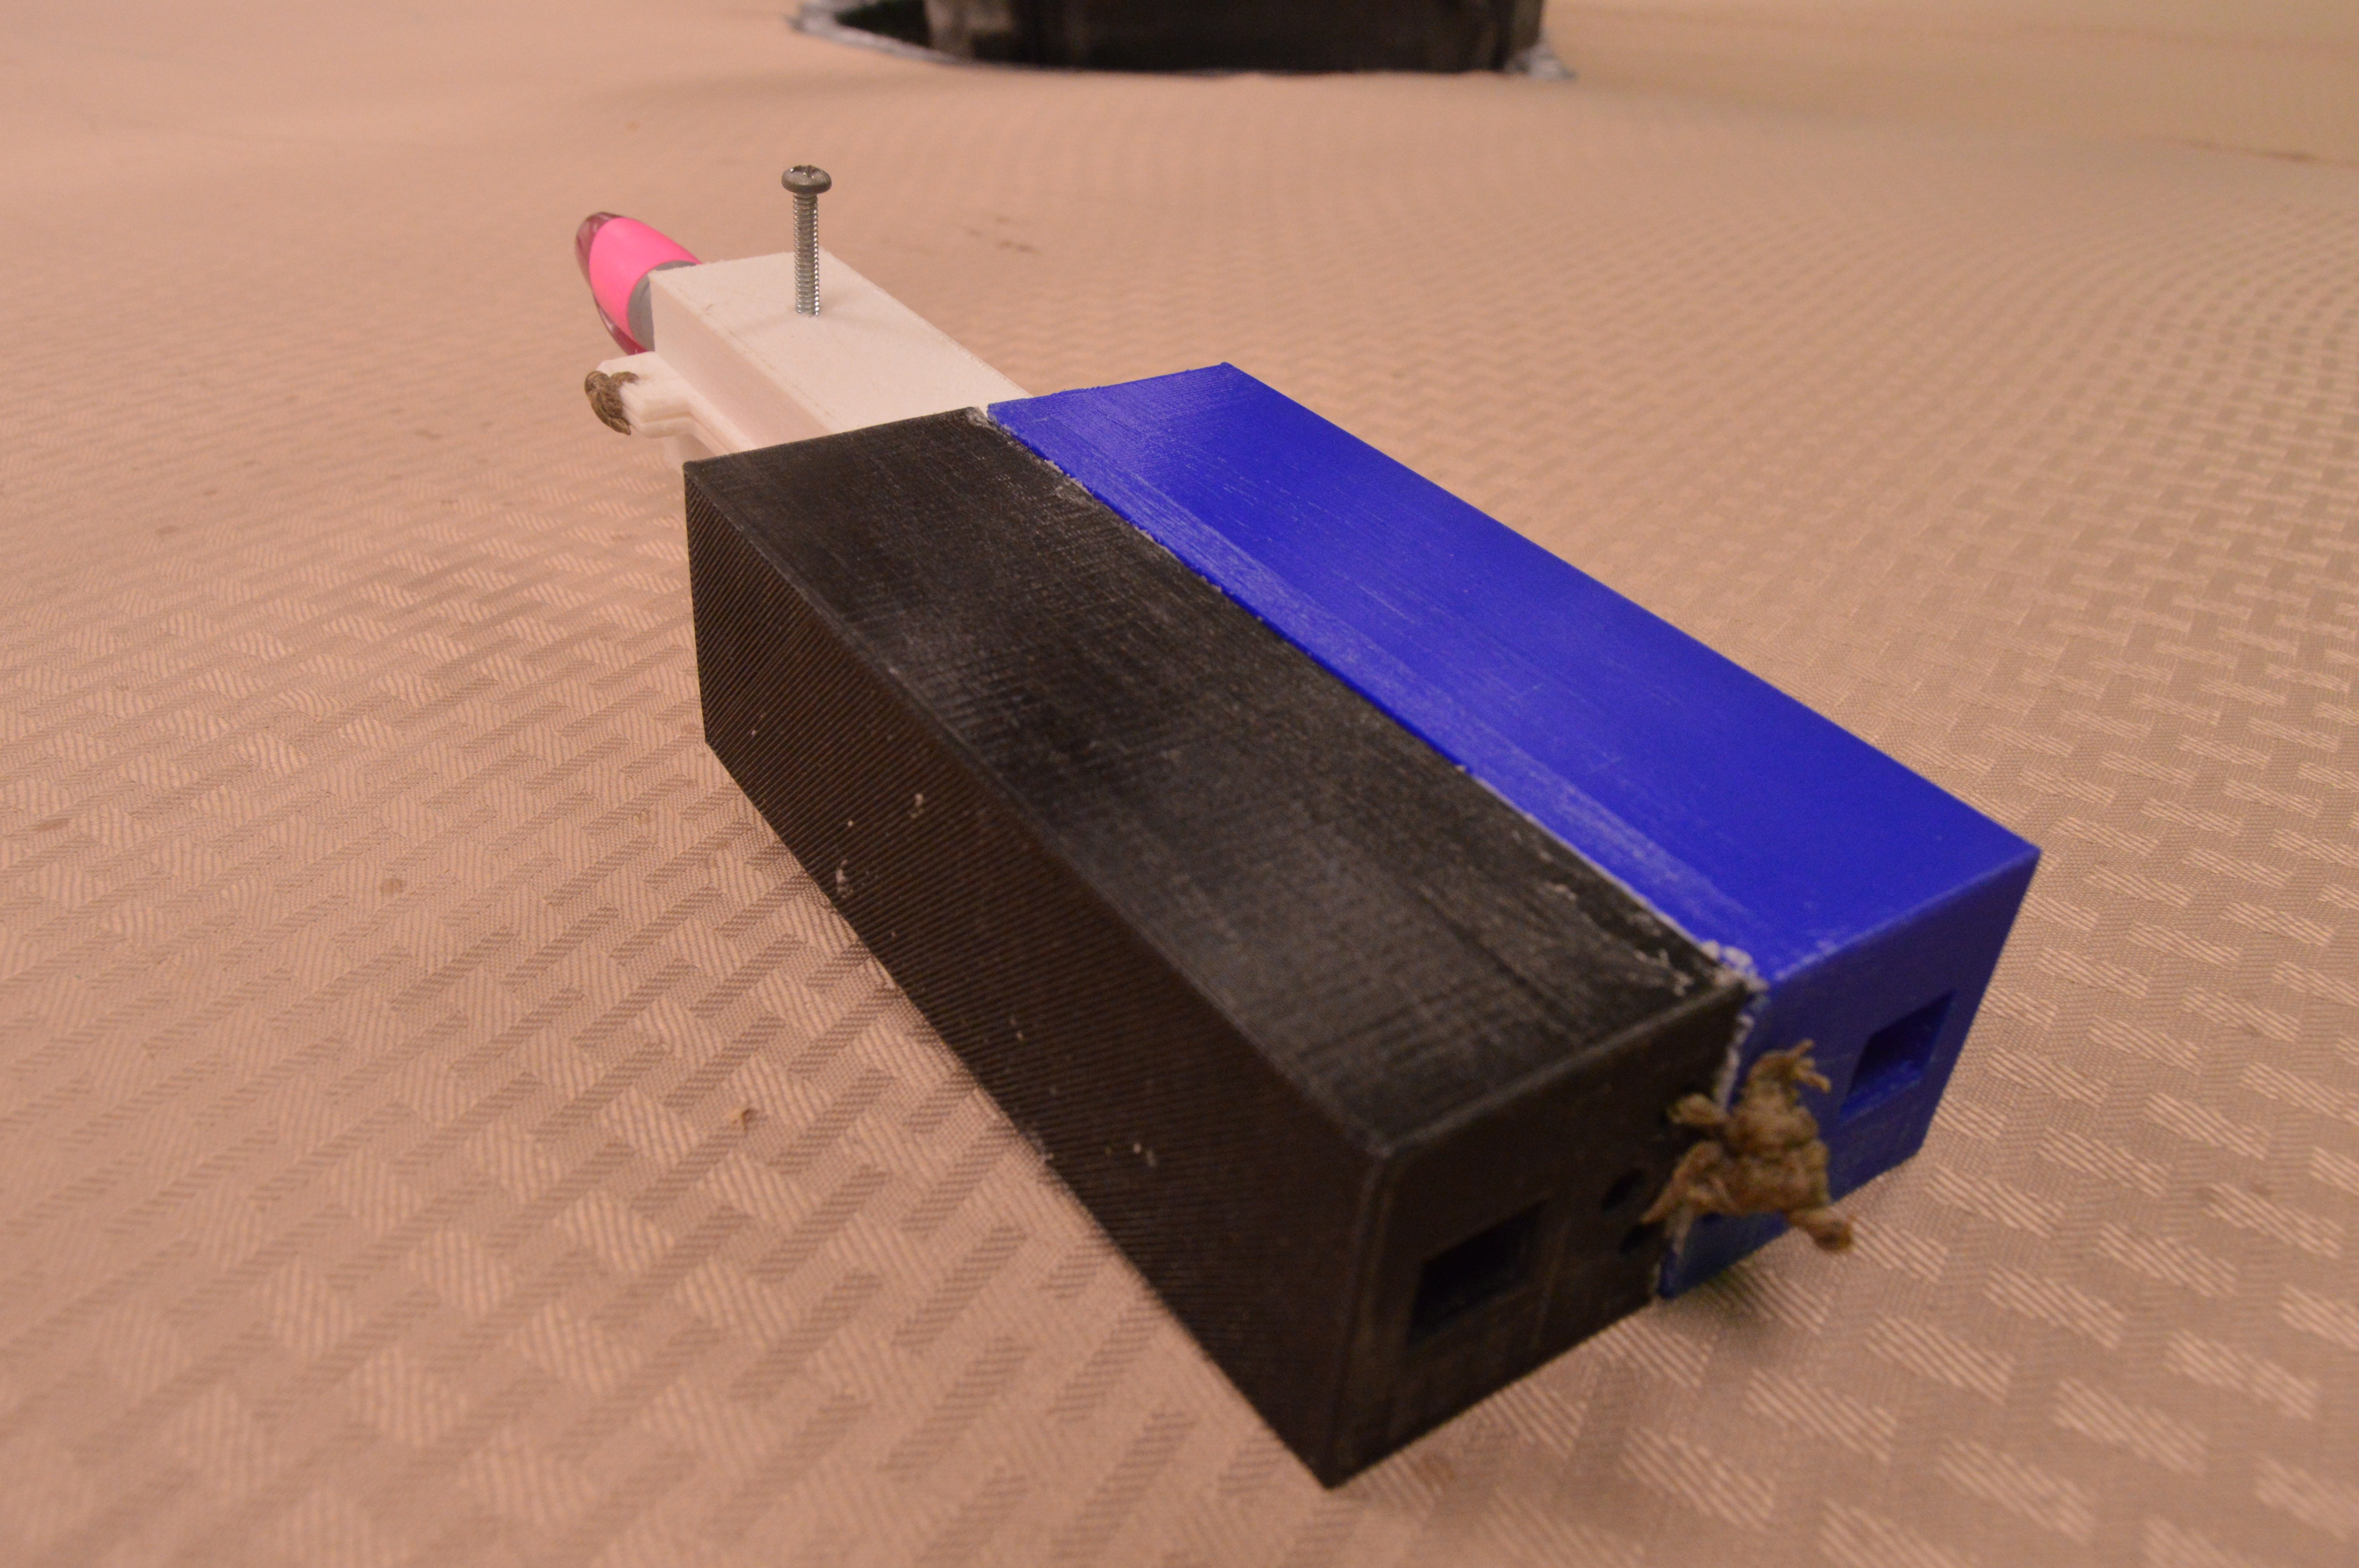
\includegraphics[width=\linewidth]{thetool.jpg}
\end{subfigure}
\hfill
\begin{subfigure}{.48\linewidth}
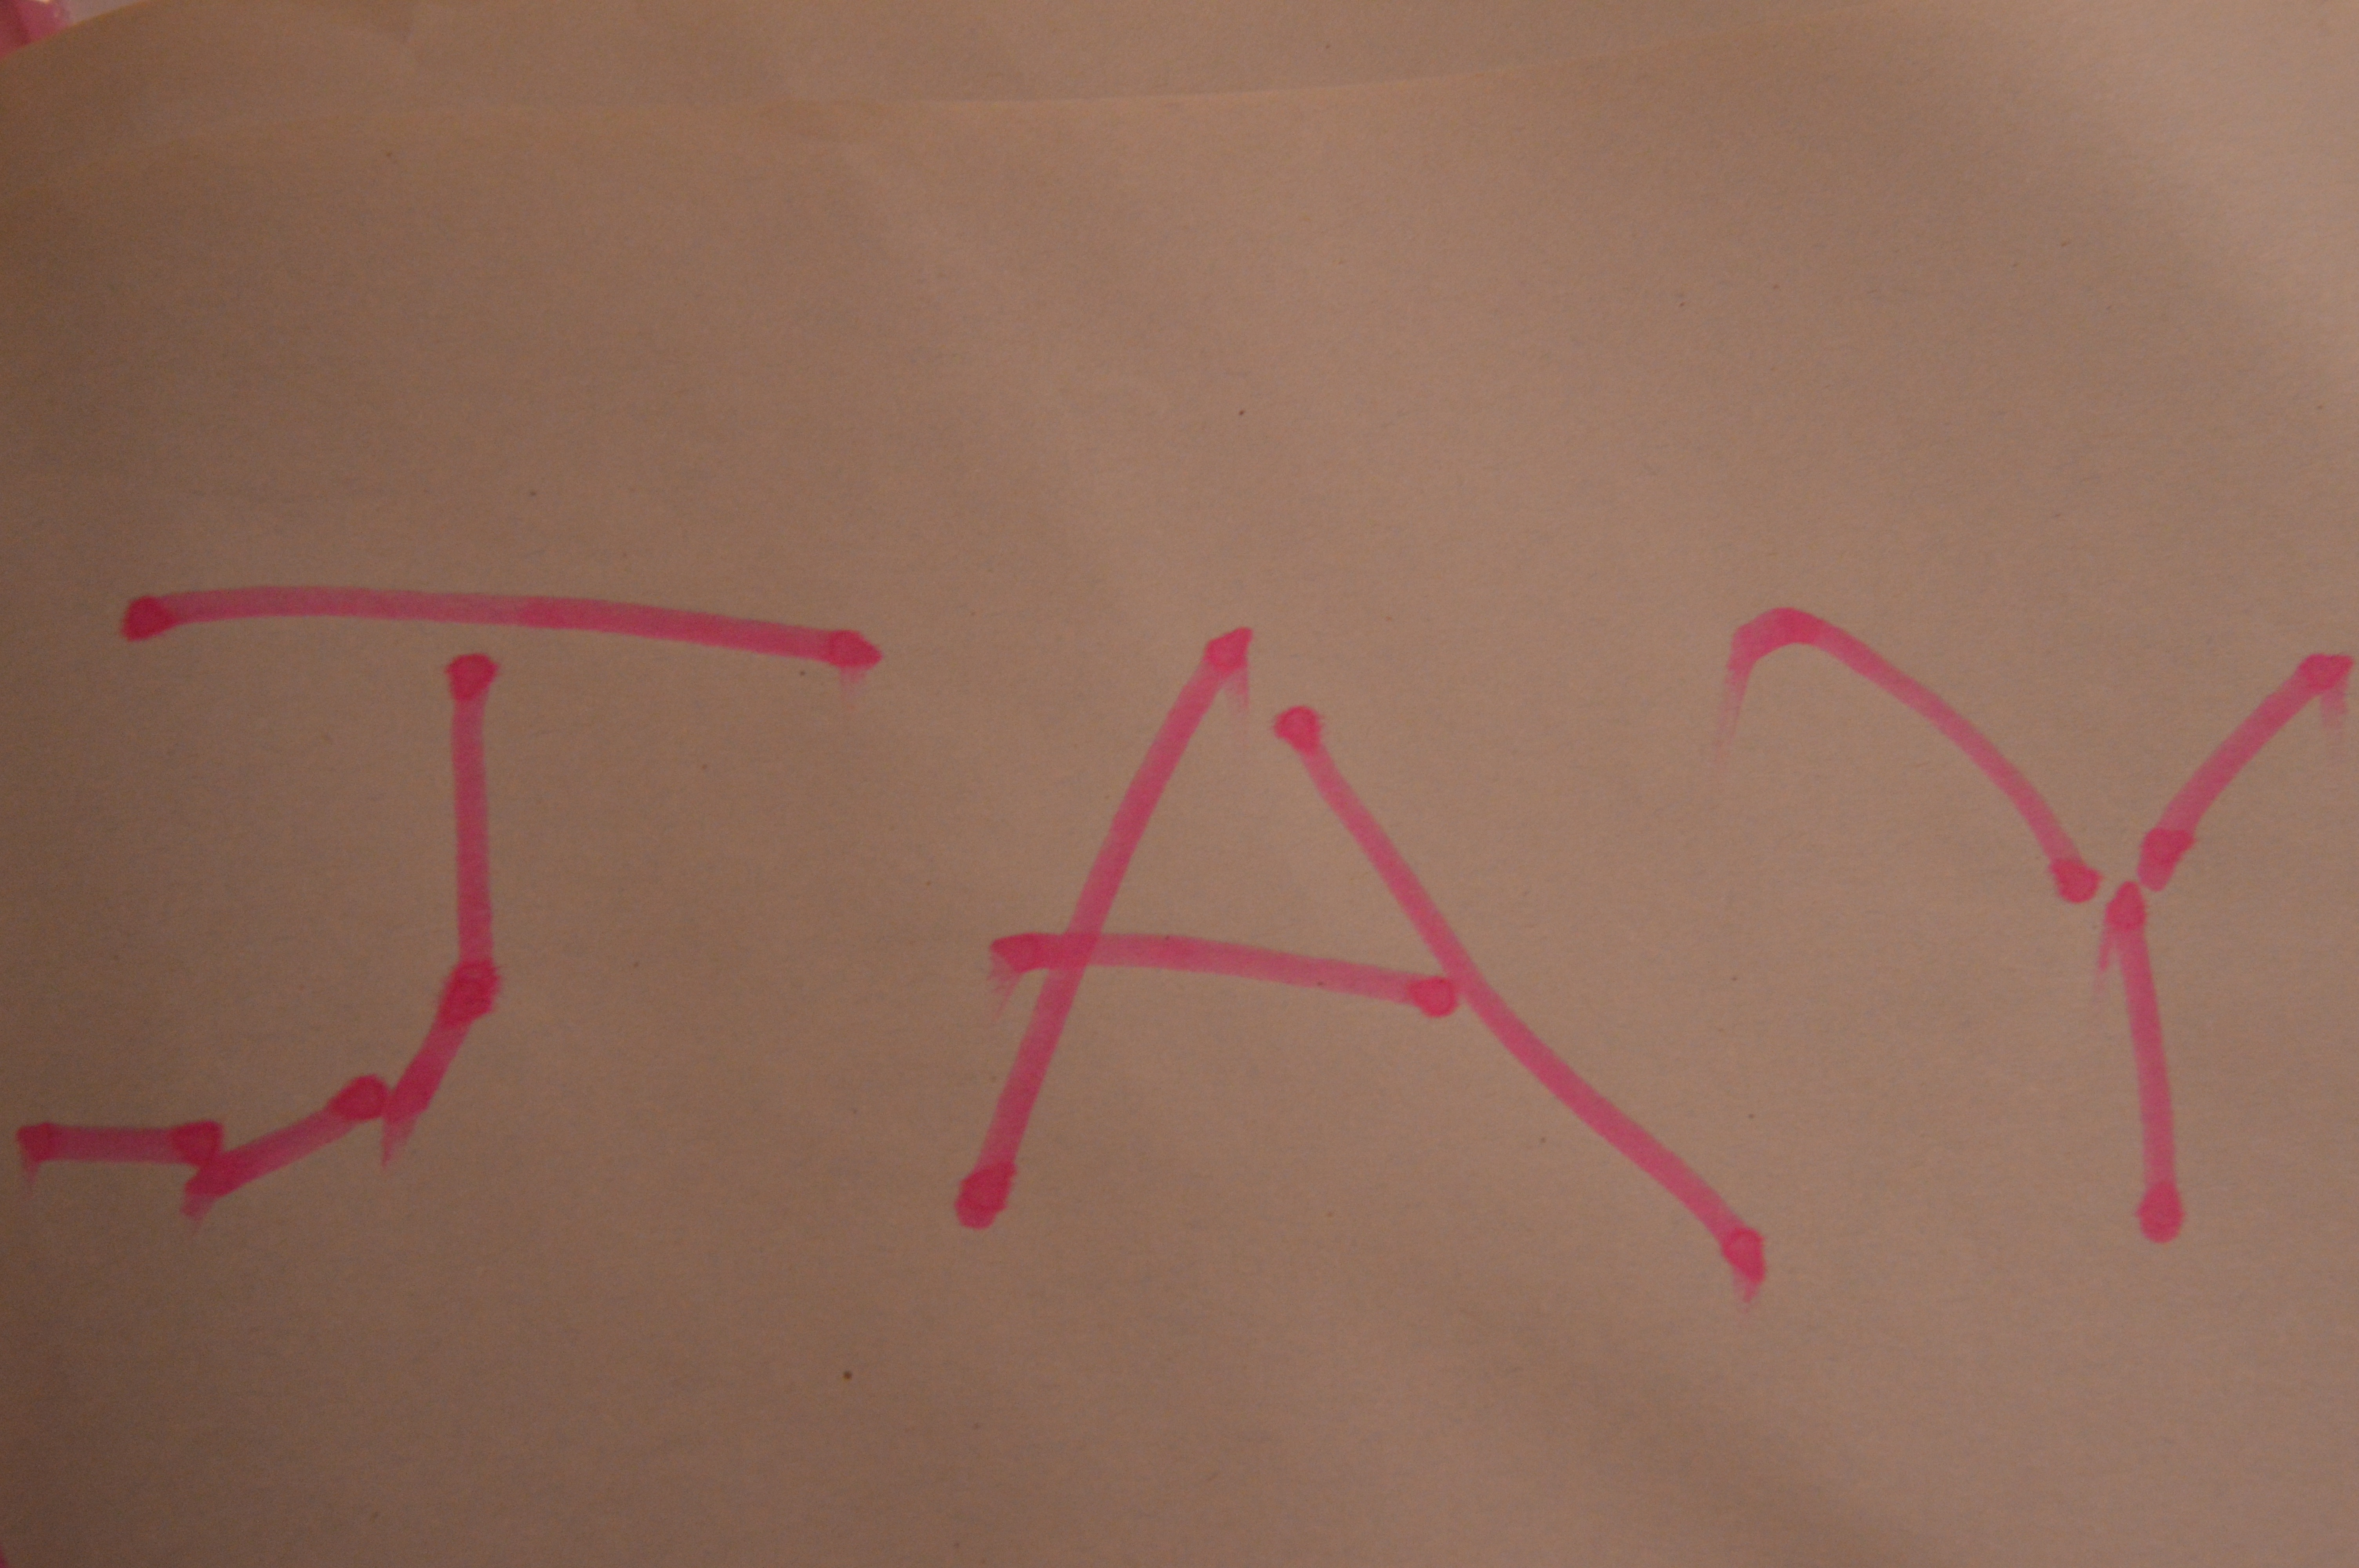
\includegraphics[width=\linewidth]{jay.jpg}
\end{subfigure}
\caption{The Writing Tool and an example of the name JAY written}
\label{tool}
\end{figure}

\section{Design}
The Writing Tool described below was specifically built for the Baxter Robot, a research and industrial robot built by Rethink Robotics, which is a humanoid robot with two seven degree-of-freedom arms, as well as many different sensing technologies. Baxter has two grippers which can open and close, which are typically used for object delivery tasks. These grippers can not properly hold a writing utensil, such as a marker, to write. Baxter easily loses its grip and it is difficult to prevent Baxter from over or under applying pressure. We have built a tool that Baxter grips in order to write. Baxter can simply slip its open grippers into the slots, and then close the grippers to apply pressure to hold onto it (see Fig \ref{wearing}). Because the writing chamber that is holding the utensil is directly in front of Baxter's end effector, the tool acts as a simple extension of Baxter's arm that allows it to write with strong control. Because of the screws on the Writing Tool, the writing utensil can sit securely inside the Writing Chamber and be accurately controlled by Baxter. Because our tool uses screws, this also allows Baxter to change writing utensils. Rather than need to build into Baxter the ability to perform the writing task, this work has looked to allow social robots to use their built in hardware and functions to use a tool that lets them perform a task it could not do otherwise. By allowing the tool to be able to be gripped and ungripped easily, engaging and disengaging with the Writing Tool can be done autonomously. The Writing Tool was created in Solidworks in order to create a 3D-printable version. Once the parts of the Writing Tool are printed out, one can assemble the Writing Tool. We also created a Python program that uses Ein in order to control the Baxter robot to perform the writing task. Ein includes a 3D discretized grid of space that the Python program uses in order to represent points in space to draw to. The included software has preprogrammed representations of all the letters of the English alphabet, capitalized (see Fig \ref{tool}). The software allows affine transformations to be applied to these representations in order to rotate, scale, and translate letters to draw. The 3D schematics, instructions for assembly, software, and further images/videos are all included in the Github repository \cite{github}.

\begin{figure}[t]
\centering
\begin{subfigure}{.48\linewidth}
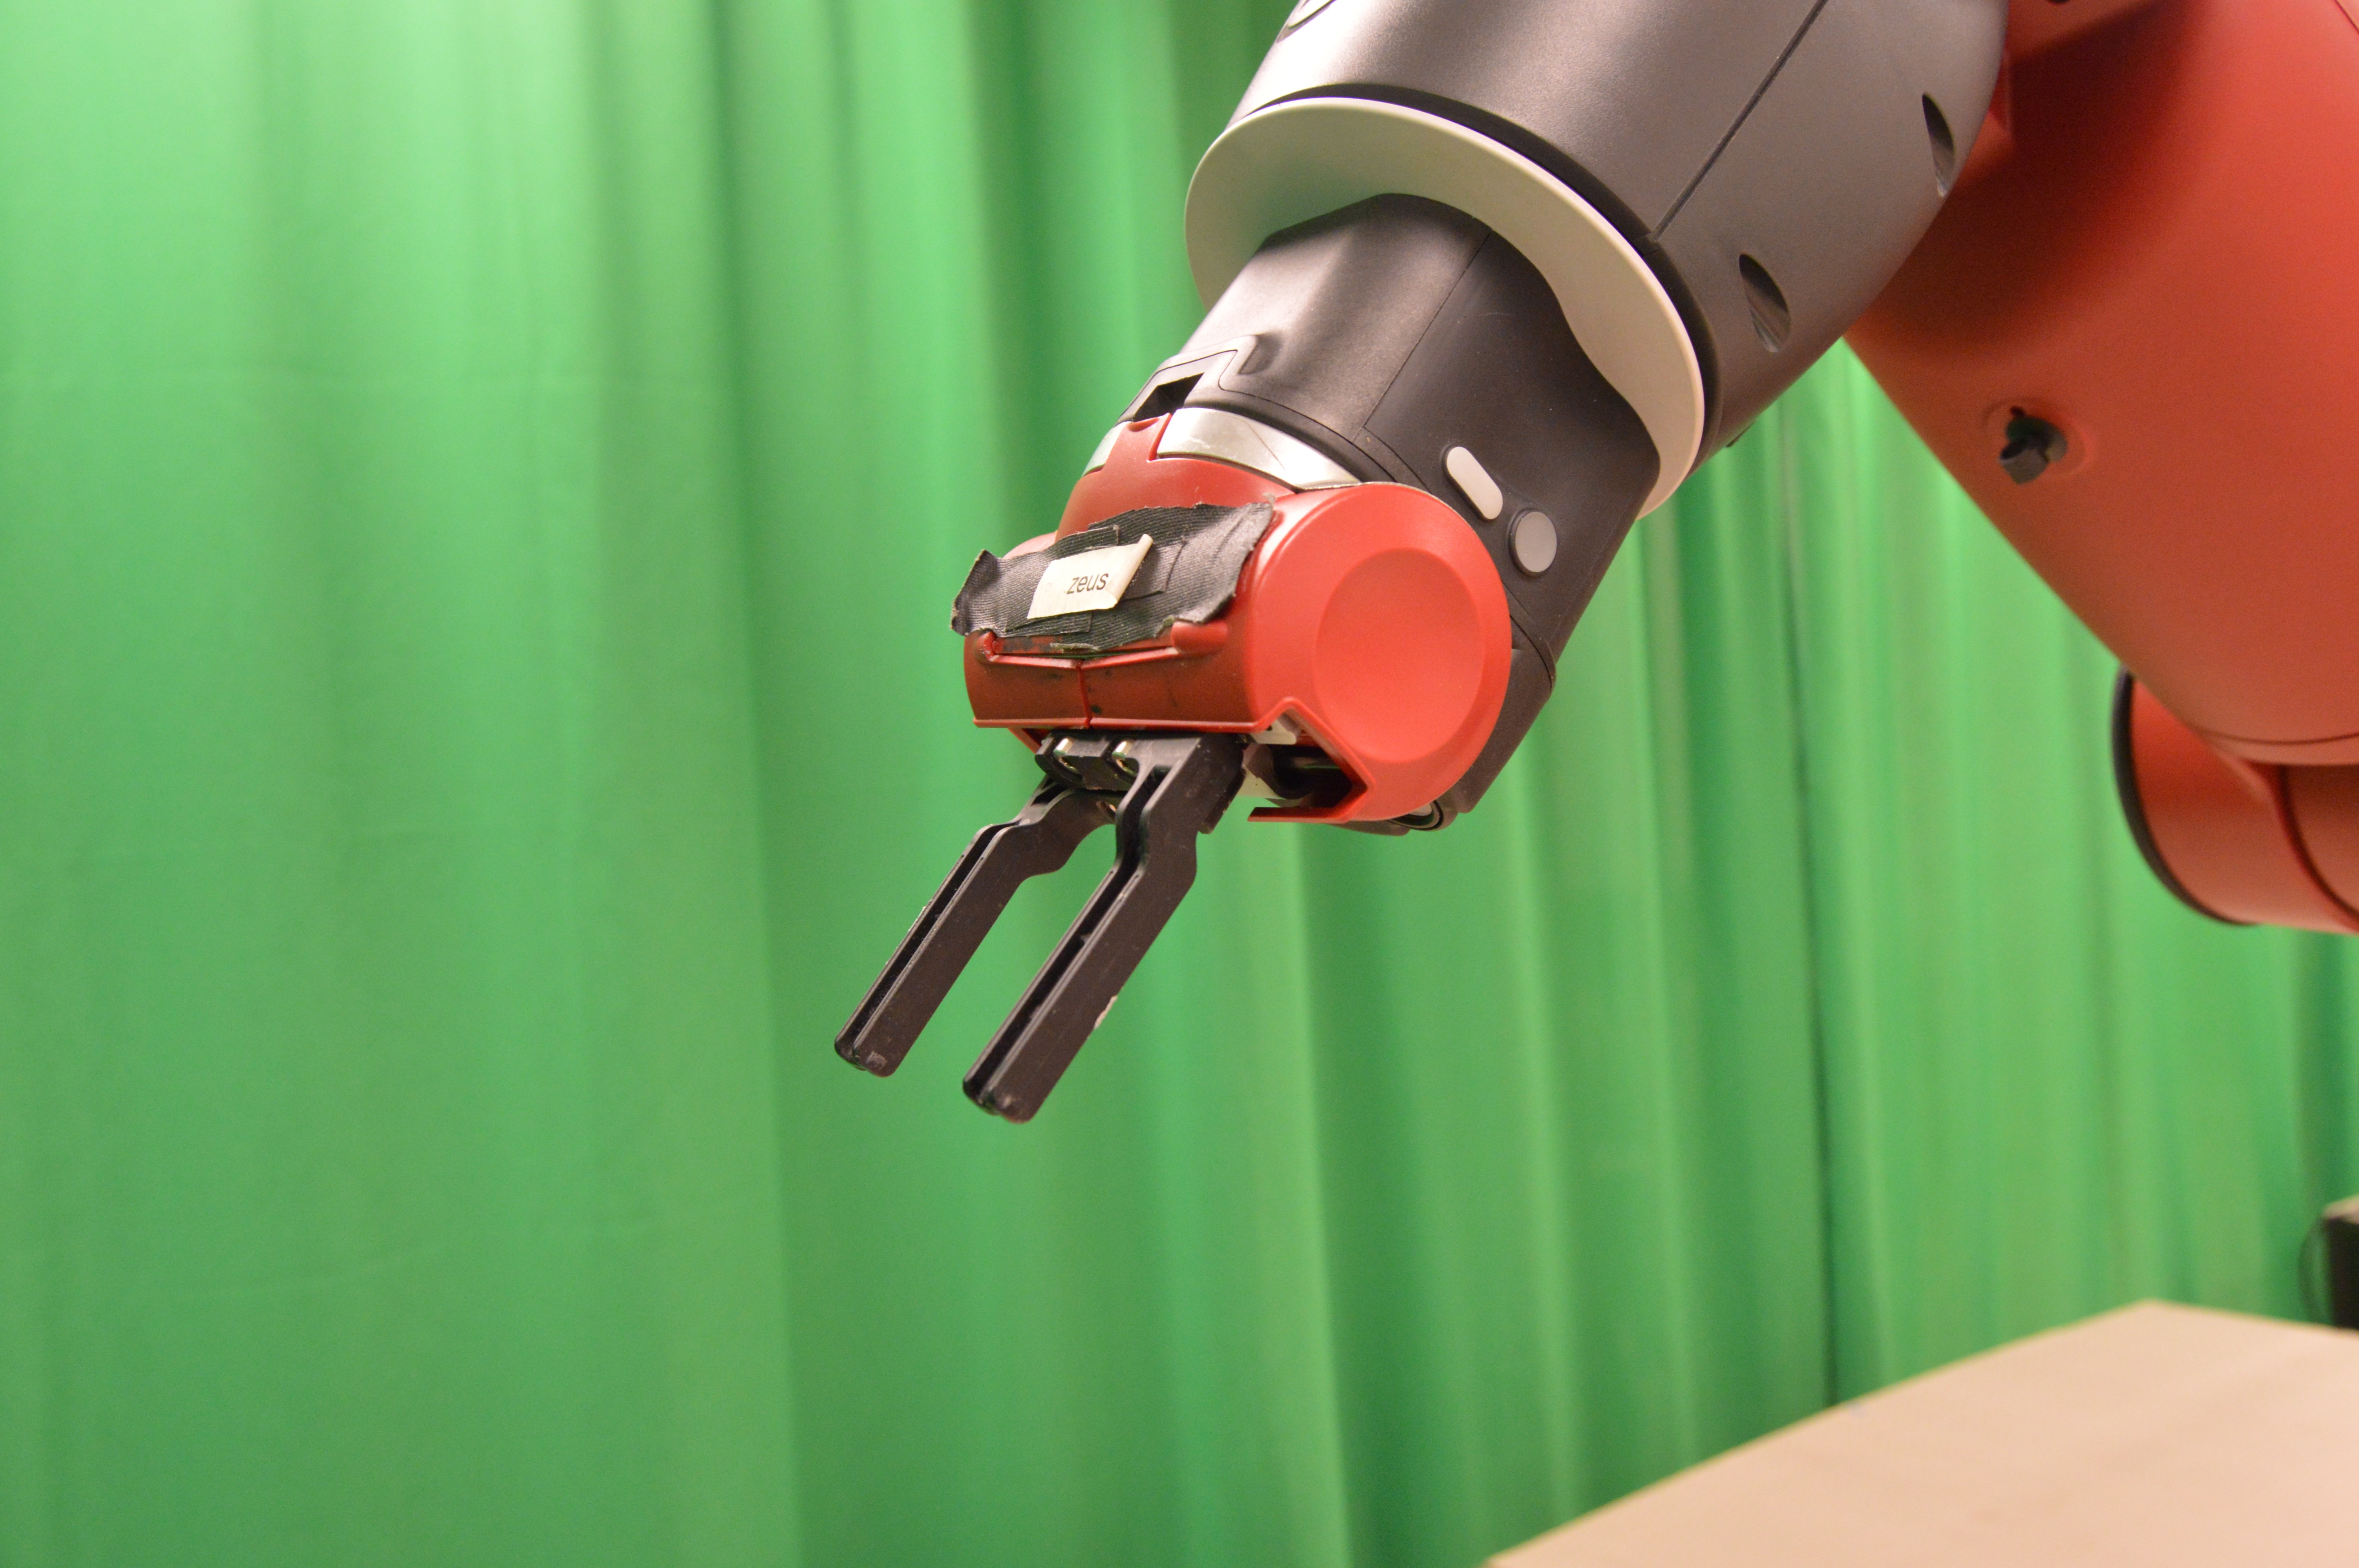
\includegraphics[width=\linewidth]{notholding.jpg}
\end{subfigure}
\hfill
\begin{subfigure}{.48\linewidth}
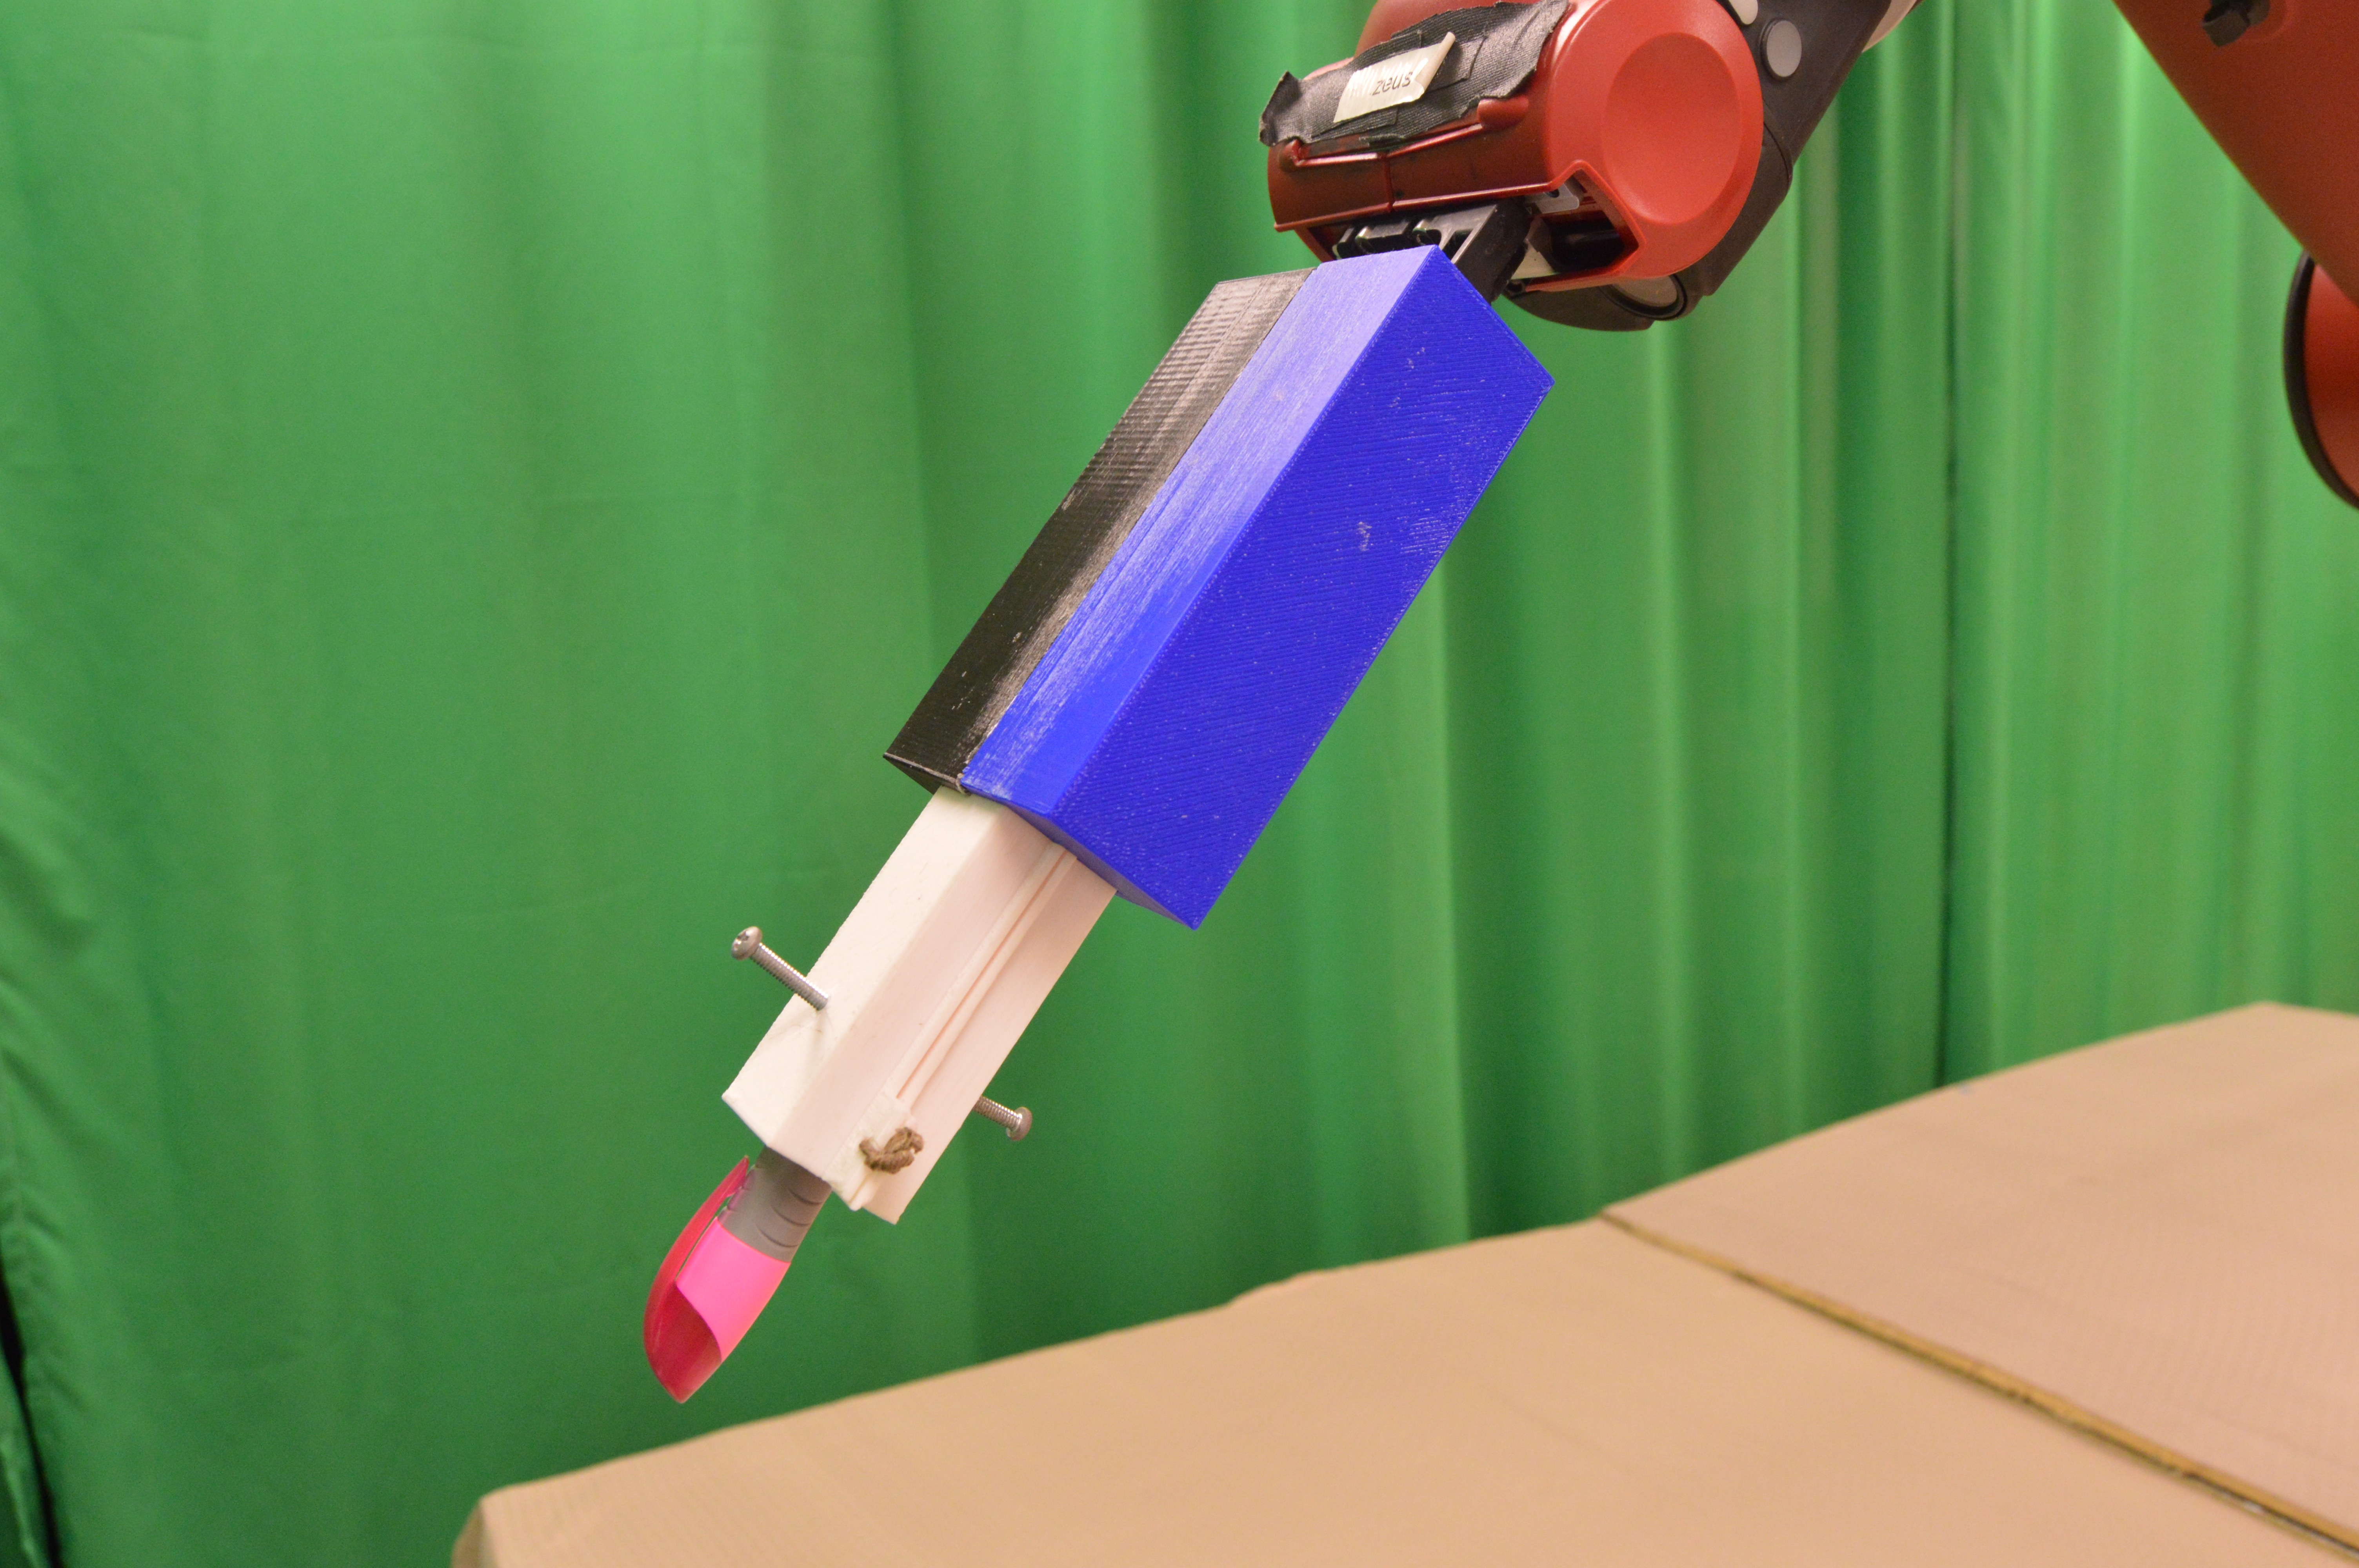
\includegraphics[width=\linewidth]{holding.jpg}
\end{subfigure}
\caption{Baxter not holding and holding the Writing Tool}
\label{wearing}
\end{figure}
The speed at which the writing tool moves has an effect on the smoothness and mark impact on the writing canvas. Because Baxter's end effector is prone to small jitters, the slower the line is drawn, the more likely the line will not be straight. However, the slower the line is drawn, the more impact the mark has on the paper due to its longer time exposure. When the drawing tool is whipped quickly, it leaves more of a streak mark than a full drawn mark. Thus, the speed is a parameter in the program that can be changed in order to get the desired results. The angle at which the writing utensil interacts with the writing canvas will determine how much of the mark is let upon it. Humans typically hold their writing utensil at an angle from the canvas when they draw. While drawing, they ``anchor'' their hand onto the canvas, which allows more fine grain control over the precision and accuracy. This ``anchoring'' is not implemented in any of the demonstrations in this work, and are all performed orthogonally with respect to the canvas. However, it is still possible to start the utensil at any degree so it can swipe the writing utensil point to point. The steeper the angle, the less fine control over the mark the robot has. In order to keep the most unified stroke marks throughout the drawing, the orientation of the writing utensil's tip is held constant throughout the stroke. This means that when the program draws a line segment between two points, it calculates the angle of the vector relative to the grid, and orients the tool to match it. This allows the same side of the writing utensil to always be applied to the canvas. However, some writing utensil are used at different orientations depending on desired effect, so one can program the writing tool to rotate throughout the stroke if desired.

\section{Possible Extensions of Work}
The better ability the robot has to have feedback to how the end effector is actually acting, the more it can self correct itself. When writing, it is important to have constant feedback in order to match the different surface properties and tension that exists throughout the canvas. In order to accommodate this, the design of the end effector tool allows for Baxter’s IR sensor to not be blocked so that the distance of the end effector to the canvas can be tracked for how much pressure the end effector tool is applying. Furthermore, since there is only one spring that sits inside the writing chamber in a very simplified domain, one can utilize basic spring physics by knowing the length of resting spring and its spring constant to see how much pressure is being applied to the canvas based on its compression. By synthesizing the IR sensor with the measurements of the spring, it is possible to create a program that measures how much pressure is currently being applied.  Because the amount of pressure that is being applied to the writing canvas from the writing utensil dictates the drawing, it is important the way that the writing utensil displaces from resting position matches what the robot is doing. If the writing chamber does not properly shift with how the robot should move it, the robot may start to make mistakes and could either push the writing utensil too hard into the writing canvas, or not enough to make a mark. Thus, the circumference of the writing chamber is in accordance with the circumference of the hole of the writing body that holds it such that the writing chamber does not have any room to shift horizontally, but can easily shift vertically in and out of the writing body to displace the spring accordingly. An interesting aspects of drawing is creating curves. In this work's software, we draw line segments between points in order to write and draw. However, many artists do not think about drawing from one point to another; they draw their stroke based on muscle memory. Because Baxter has a higher degree of freedom than most writing robots, the authors wonder if deep learning could be applied to this area of robotics in order to learn what servo angles are needed to be assumed in order to solve drawing curves and line segments. This could allow for Baxter to have very unique and natural looking drawing marks, rather than the less natural looking ones that are currently drawn. By using feedback such as IR and an understanding of how the spring is working inside the Writing Tool, different methods of deep learning could possibly help solve the optimal paths for Baxter to move its arm in order to draw and write.
%\section{References}

%%%%%%%%%%
% References and End of Paper
\bibliographystyle{aaai}
{\small
\bibliography{sources} 
}

\end{document}
